% ----------------------------------------------------------------------
%  Pracovní úkoly
% ----------------------------------------------------------------------
\section{Pracovní úkoly}

\begin{enumerate}
\item Studium lomových ploch pomocí SEM.

\item Měření střední velikosti zrna polykrystalického vzorku. K vyhodnocení snímku ze scanovacího elektronového mikroskopu použijte kruhovou metodu.

\item Určení frakčního objemu dané fáze ve vícefázovém materiálu. Použijte specializované programové vybavení pro obrazovou analýzu.
\end{enumerate}

% ----------------------------------------------------------------------
%  Teoretická část
% ----------------------------------------------------------------------
\section{Teoretická část}

Chyba je spočtena pomocí metody přenosu chyb \cite{bib:metoda-prenosu-chyb} jako

\begin{equation}
    \sigma = \sqrt{\sum^n_{i=1} \left( \frac{\partial f}{\partial x_i} \right)^2 \sigma^2_{x_i}}
\end{equation}

% ----------------------------------------------------------------------
%  Výsledky a zpracování měření
% ----------------------------------------------------------------------
\section{Výsledky a zpracování měření}

\subsection{Studium lomových ploch}

Studovali jsme intermetalickou slitinu na bázi $Fe_3Al$ v závislosti na teplotě. Zajímala nás morfologie povrchu, proto jsme zvolili měření sekundárních elektronů. Závislost na teplotě jsme získali proměřením dvou vzorků, jeden tažený při pokojové teplotě, druhý při teplotě 700 °C. Na obrázku \ref{fig:lom_rt_combined} (vlevo) je snímek z elektronového mikroskopu vzorku taženého při pokojové teplotě, na obrázku \ref{fig:lom_rt_combined} (vpravo) je detailní snímek ve větším zvětšení. 

\begin{figure}[!h]
    \centering
    \begin{minipage}[b]{0.48\linewidth}
        \centering
        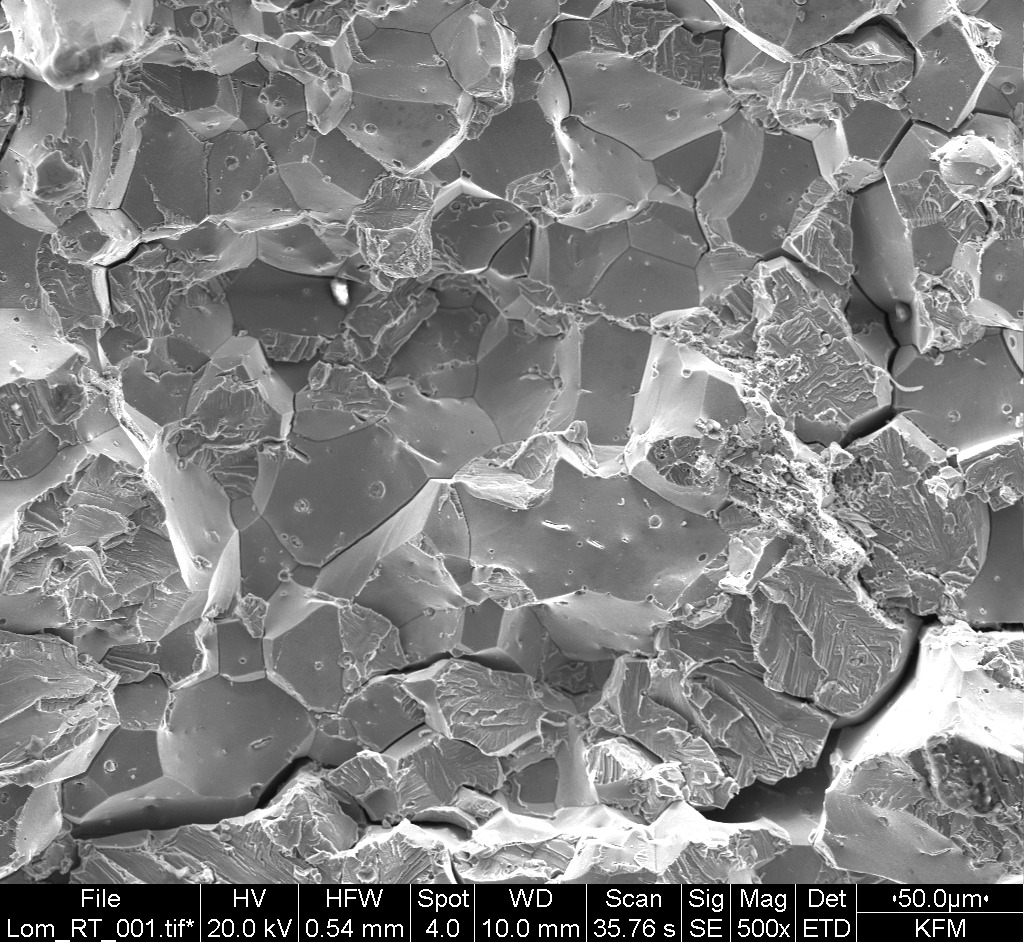
\includegraphics[width=\linewidth]{A18 - SEM/Lom_RT_001.jpg}
    \end{minipage}
    \hfill
    \begin{minipage}[b]{0.48\linewidth}
        \centering
        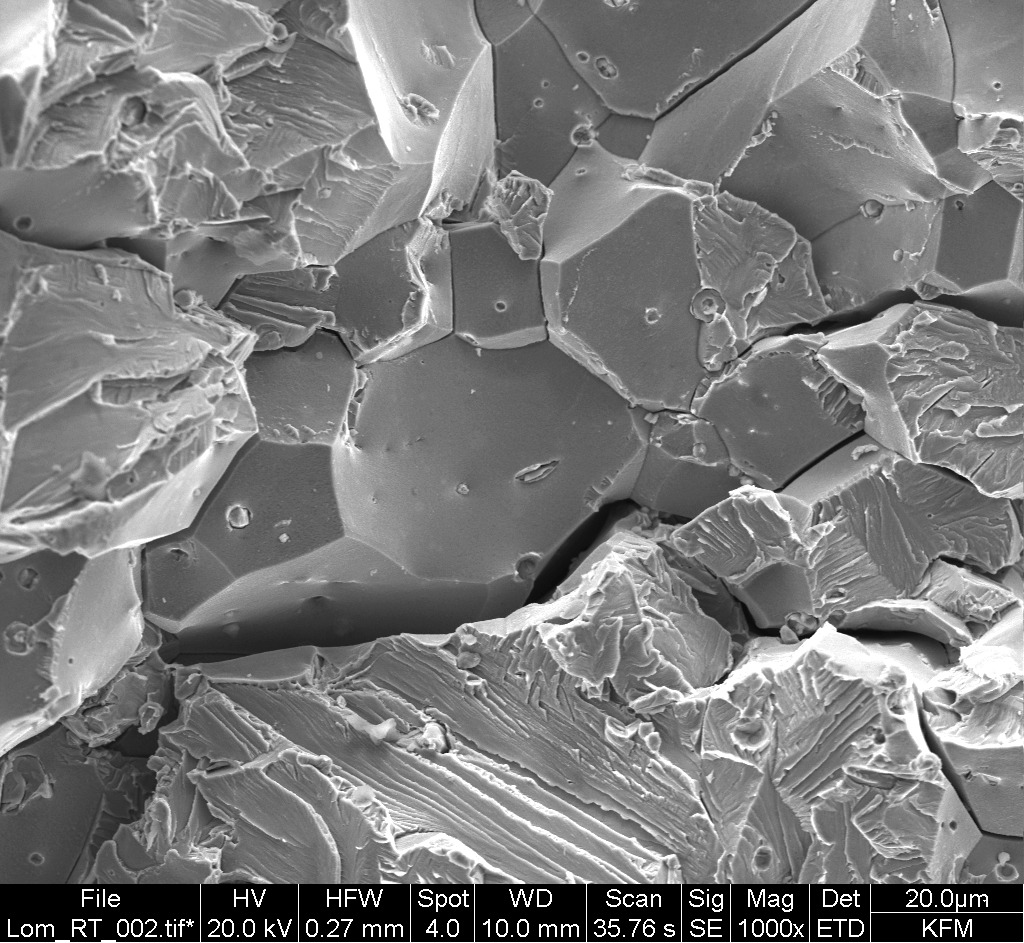
\includegraphics[width=\linewidth]{A18 - SEM/Lom_RT_002.jpg} % uprav dle potřeby
    \end{minipage}
    \caption{Snímky vzorku taženého při pokojové teplotě – vpravo s větším zvětšením}
    \label{fig:lom_rt_combined}
\end{figure}

Zvětšení uvedené v legendě pod obrázkem ztrácí význam, protože se jedná o poměř mezi šířkou velikosti okna v měřícím programu a šířkou měření vzorku. Legendu jsme však zanechali pro zachová ostatních parametrů. Vidíme, že se jedná o křehký lom. Lomová plocha se nachází mezi jednotlivými zrny, které jsme schopni na snímku odlišit. Tento lom se nazývá interkrystalický. V některých částech nedochází k oddělení sousedních zrn, ale k přelomení zrn daný geometrií zrn, kde je přelomení zrna přirozenější, než jejich oddělování. Takovýto děj označujeme jako transkrystalický lom. Pokud bychom se podívali na opačnou stranu původního materiálu (před přetržením), viděli bychom negativ zobrazeného snímku. Obě části by do sebe zapadly.

Podobně na snímku \ref{fig:lom_700_combined} pozorujeme vzorek tažený při teplotě 700 °C.

\begin{figure}[!h]
    \centering
    \begin{minipage}[b]{0.48\linewidth}
        \centering
        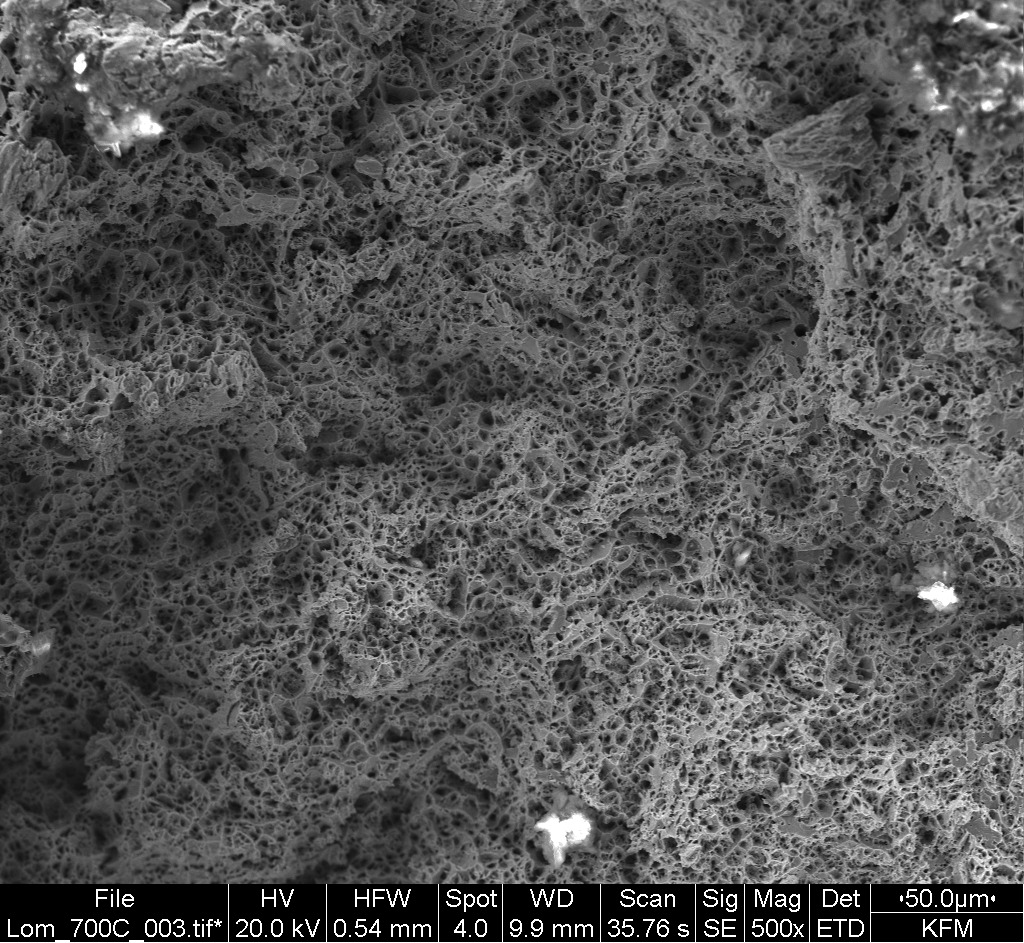
\includegraphics[width=\linewidth]{A18 - SEM/Lom_700C_003.jpg}
    \end{minipage}
    \hfill
    \begin{minipage}[b]{0.48\linewidth}
        \centering
        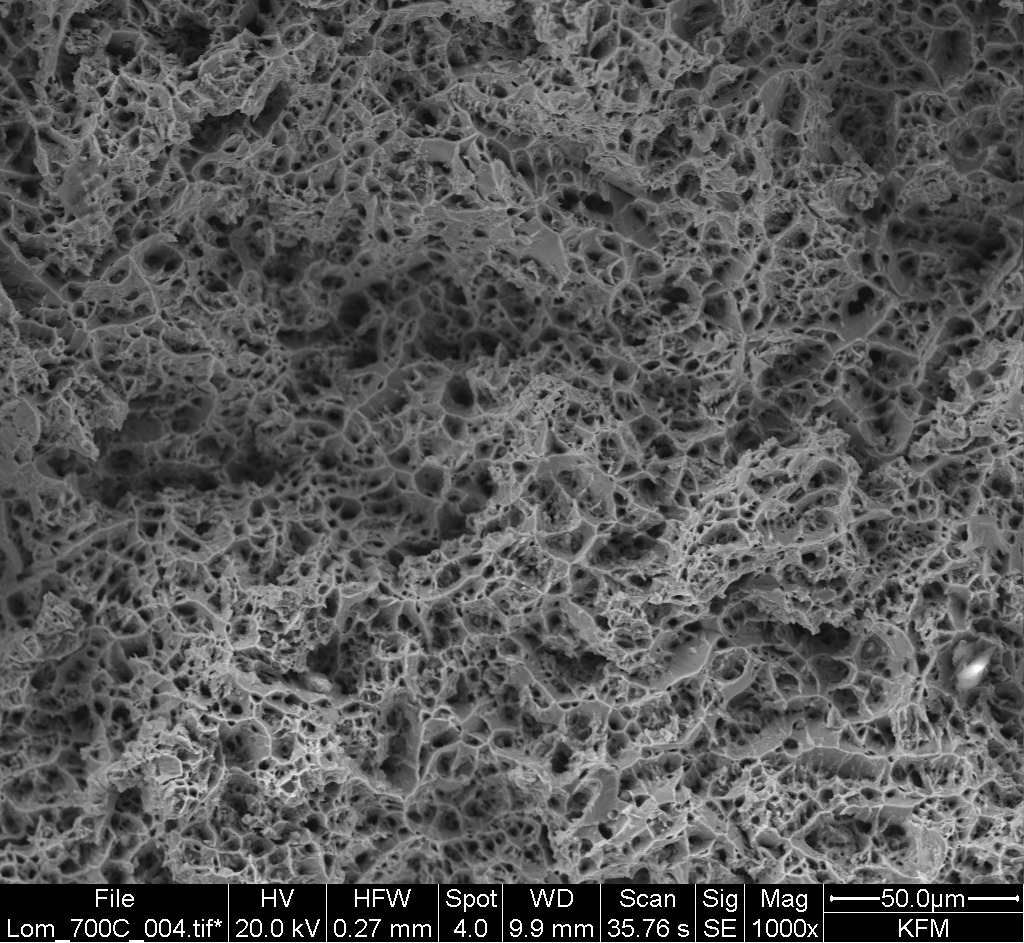
\includegraphics[width=\linewidth]{A18 - SEM/Lom_700C_004.jpg} % uprav dle potřeby
    \end{minipage}
    \caption{Snímky vzorku taženého při pokojové teplotě – vpravo s větším zvětšením}
    \label{fig:lom_700_combined}
\end{figure}

V tomto případě, na rozdíl od předchozího vzorku, pozorujeme tzv. tvárný důlkový lom. Dochází zde k velké nevratné plastické deformaci. Během tažné deformace postupně dochází k přetržení v určitých místech, ostatní části se stále plasticky deformují. Přetržených míst postupně přibývá, až se slitina přetrhne celá. Na snímku proto vidíme místa s vyššími a nižšími poklesy. Z tohoto důvodu bychom na opačné části slitiny viděli identický (alespoň velmi podobný) tvar jako v našem případě.

\subsection{Střední velikost zrna}

Pro měření střední velikosti zrna jsme využili metodu zpětně odražených elektronů. Sledovali jsme strukturu a vyhotovili čtyři snímky polykrystalického vzorku.

\begin{figure}[!h]
    \centering
    \begin{minipage}[b]{0.48\linewidth}
        \centering
        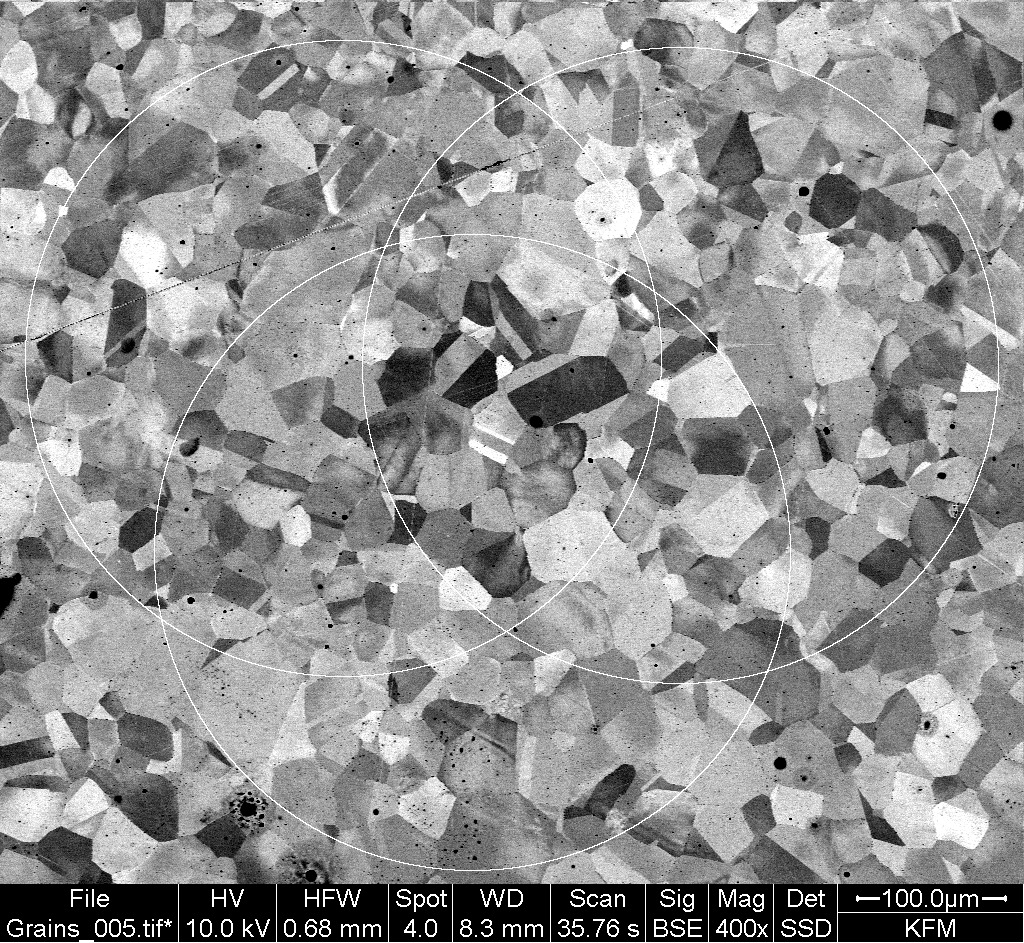
\includegraphics[width=\linewidth]{A18 - SEM/Grains_005_circ.jpg}
        \label{fig:img1}
    \end{minipage}
    \hfill
    \begin{minipage}[b]{0.48\linewidth}
        \centering
        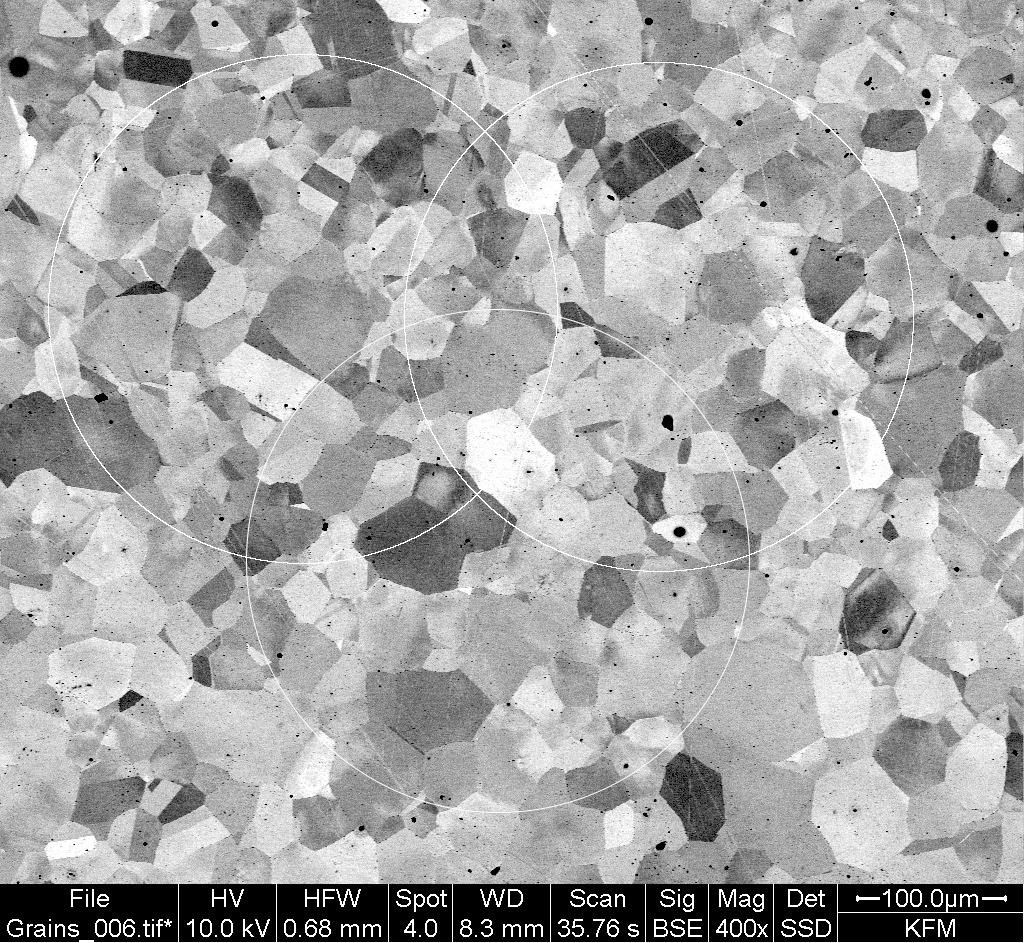
\includegraphics[width=\linewidth]{A18 - SEM/Grains_006_circ.jpg}
        \label{fig:img2}
    \end{minipage}
    
    \vspace{0.5em} % mezera mezi řádky

    \begin{minipage}[b]{0.48\linewidth}
        \centering
        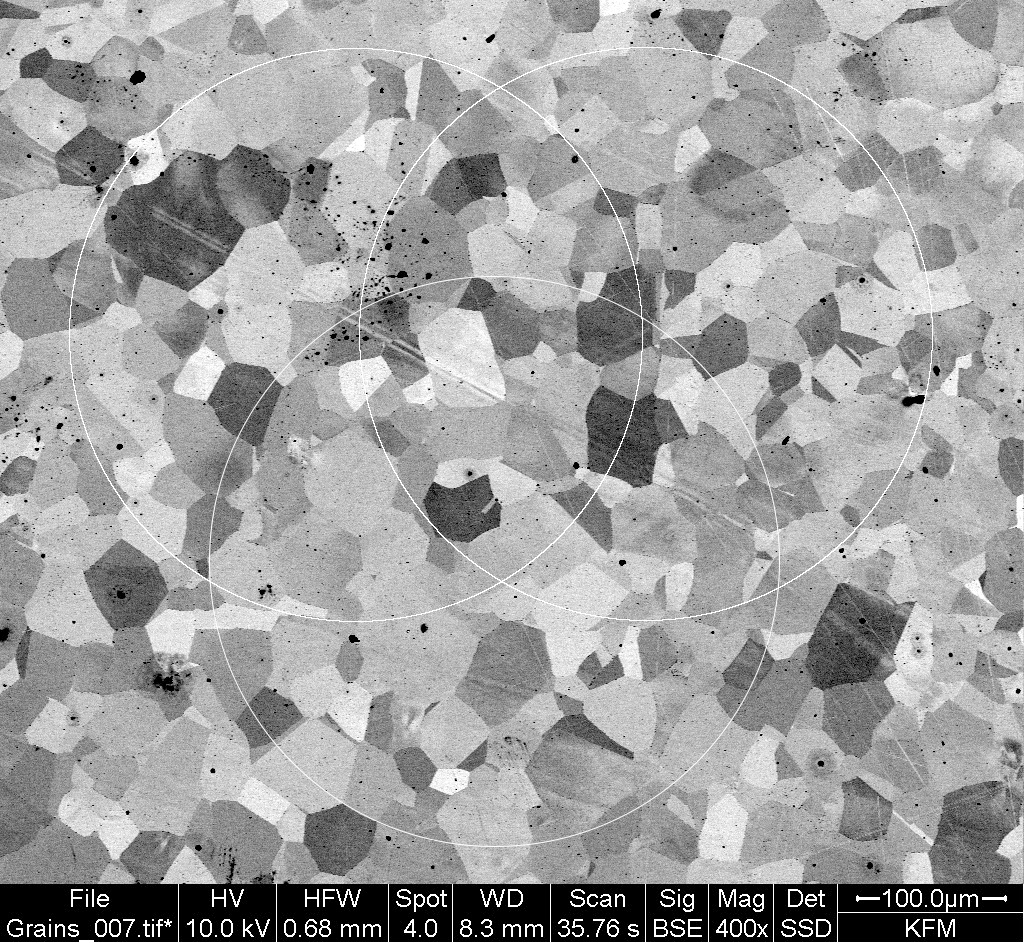
\includegraphics[width=\linewidth]{A18 - SEM/Grains_007_circ.jpg}
        \label{fig:img3}
    \end{minipage}
    \hfill
    \begin{minipage}[b]{0.48\linewidth}
        \centering
        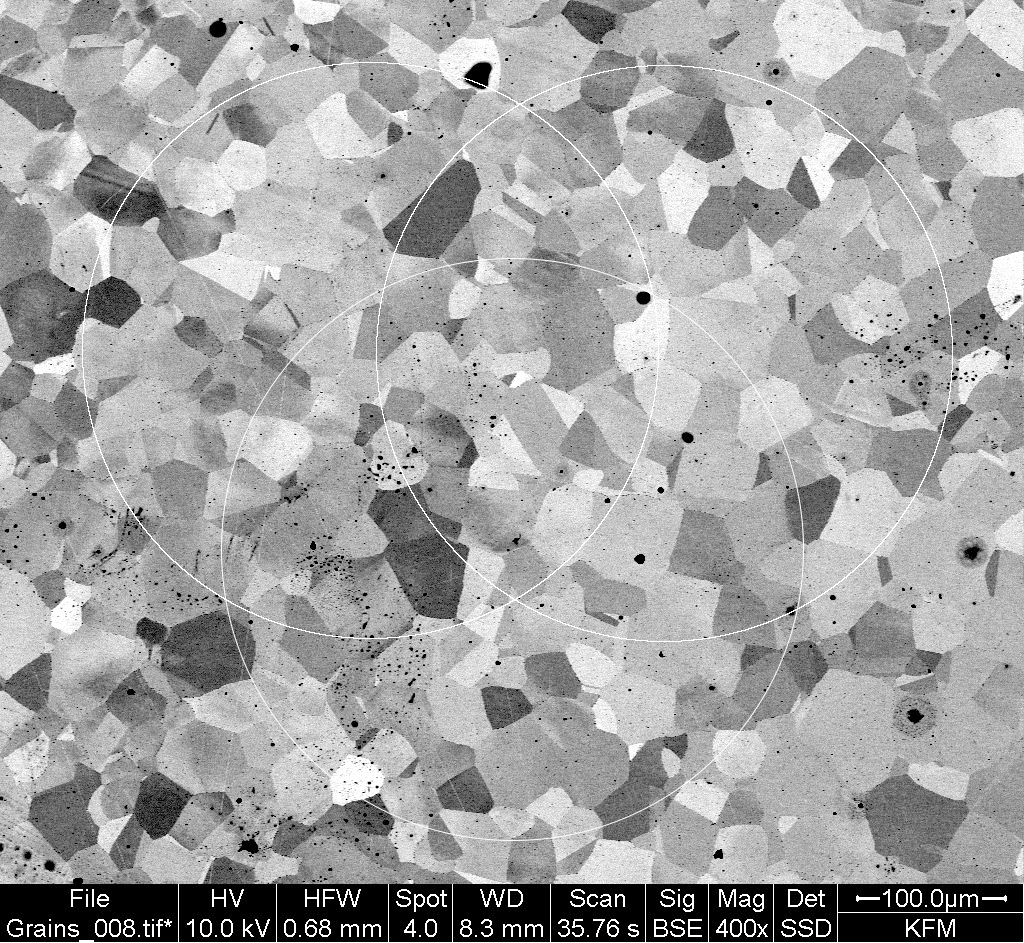
\includegraphics[width=\linewidth]{A18 - SEM/Grains_008_circ.jpg}
        \label{fig:img4}
    \end{minipage}

    \caption{Snímky polykrystalického vzorku }
    \label{fig:lom_rt_all}
\end{figure}


    
% ----------------------------------------------------------------------
%  Diskuse výsledků
% ----------------------------------------------------------------------			
\section{Diskuse výsledků}

Příčný lom



% ----------------------------------------------------------------------
%  Závěr
% ----------------------------------------------------------------------
\section{Závěr}
